Najstarszym synem Walentego i Antoniny Głąbów był Jan (ur. 10 IX 1898 r. w Mirowie).

\begin{figure}[!h]
\begin{center}
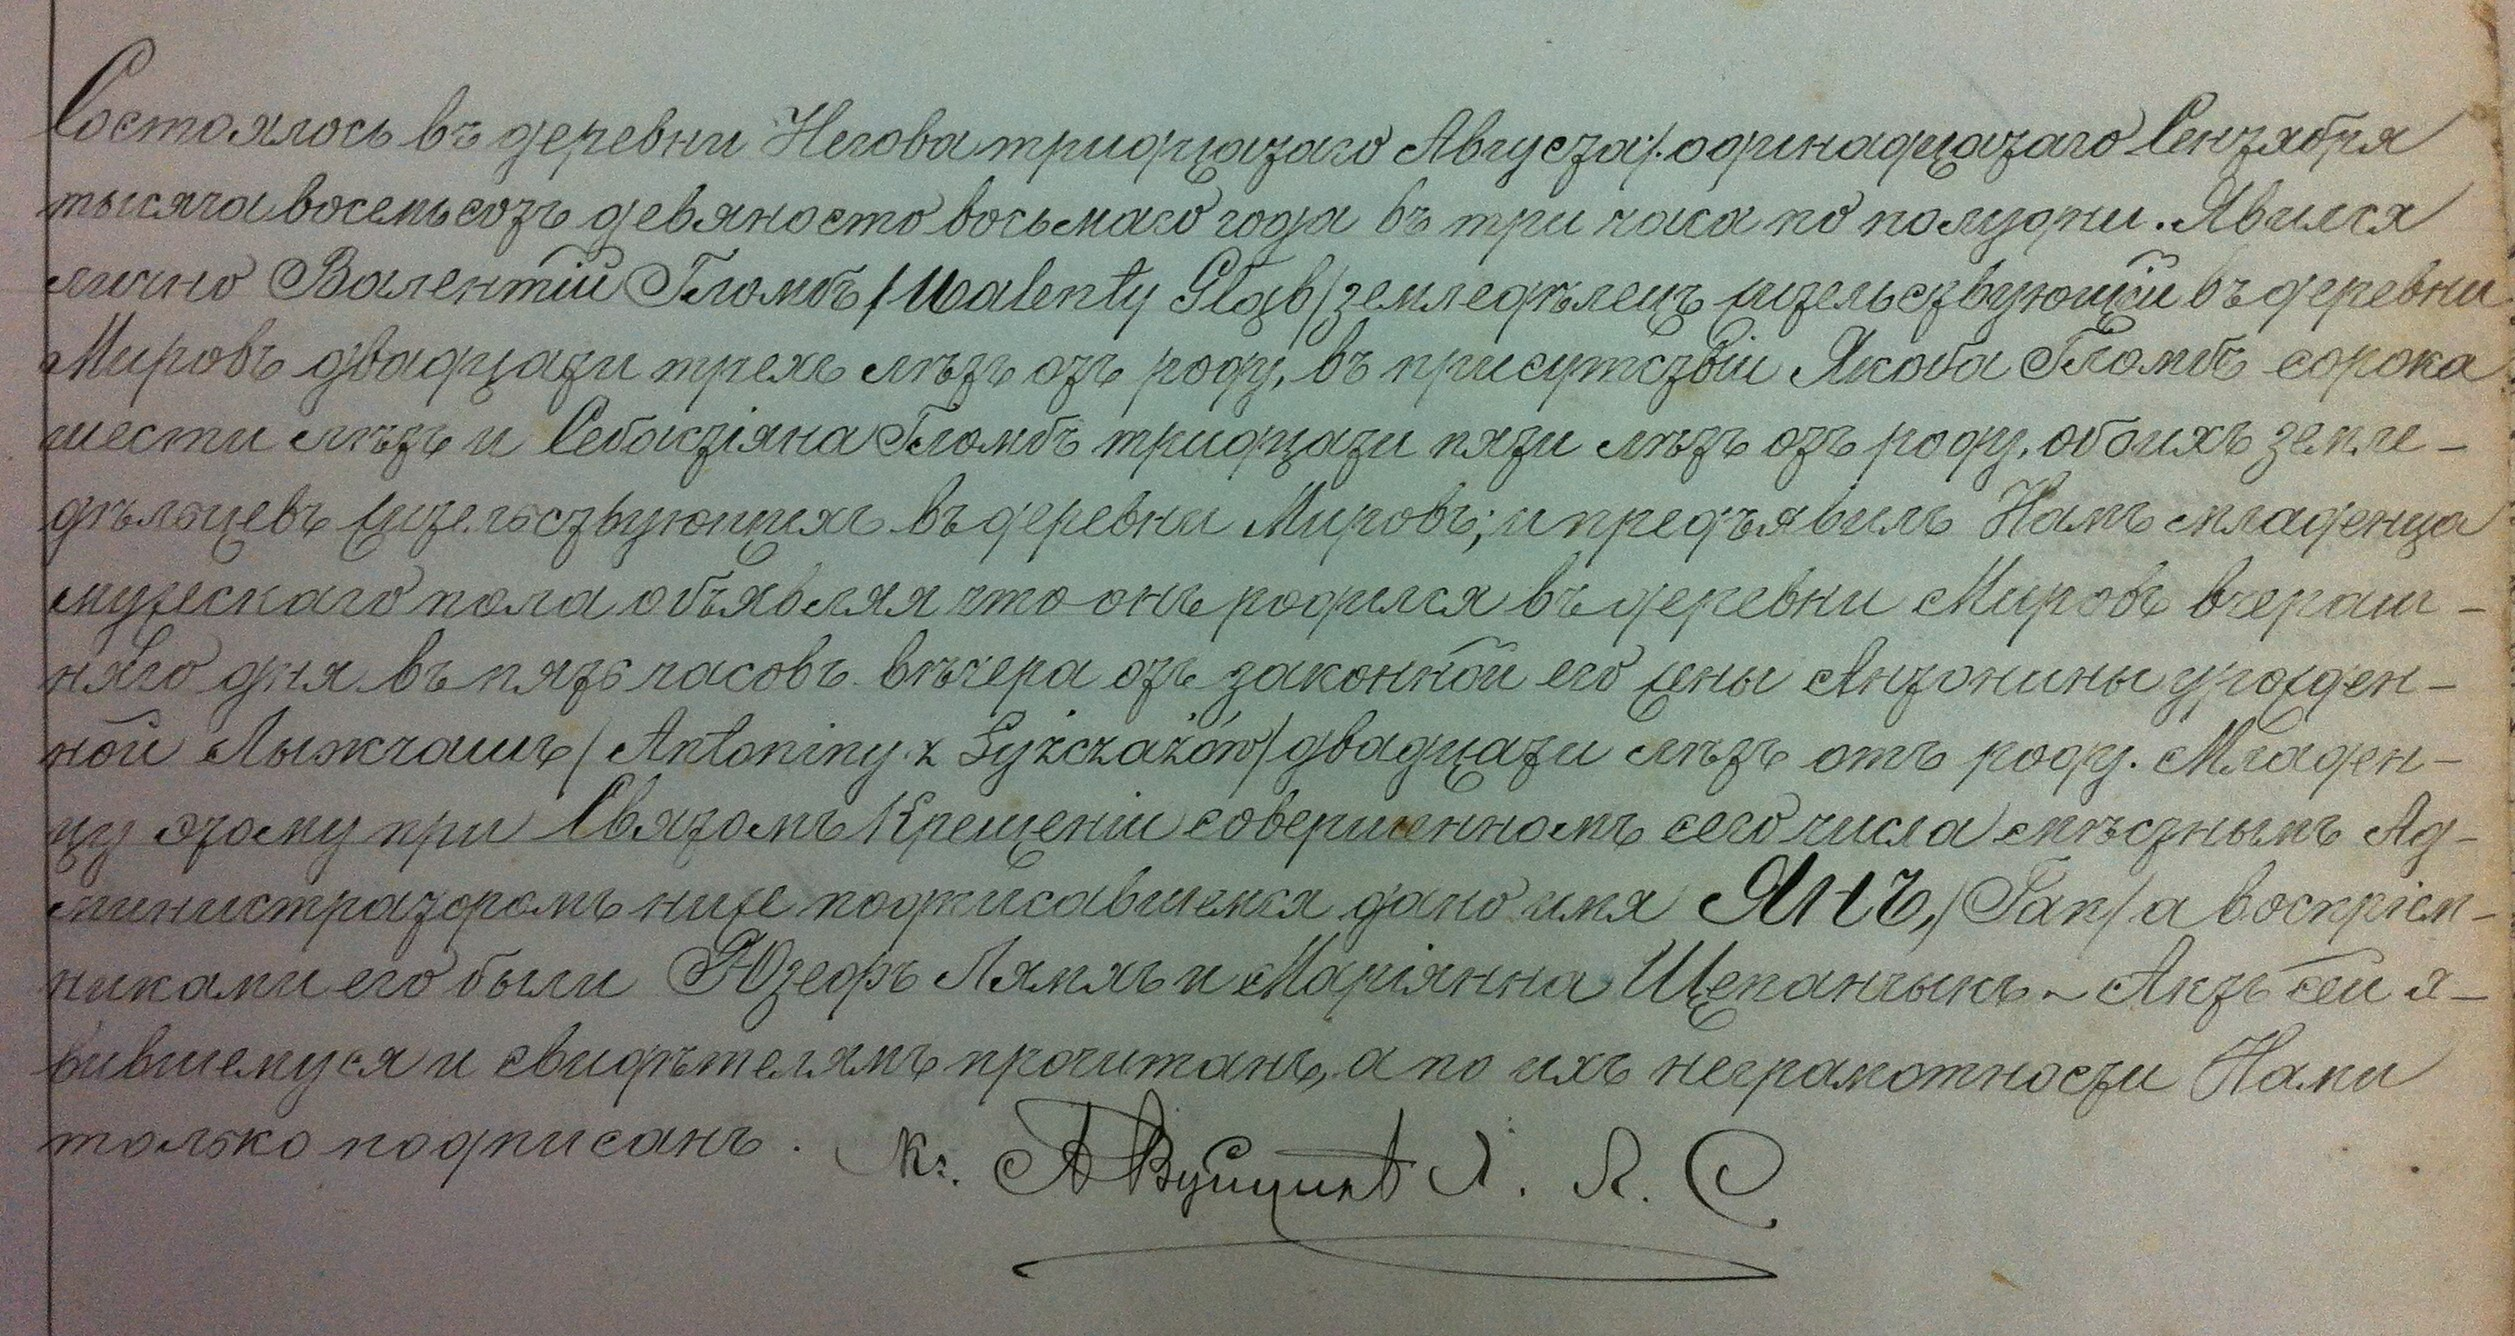
\includegraphics[width=0.8\textwidth]{zdjecia/akt_urodzenia_jana_glaba.jpg}
\caption[Akt urodzenia Jana Głąba]{Akt urodzenia Jana Głąba, syna Walentego i Antoniny z domu Łyszczarz}
\label{rys:akt_urodzenia_jana_glaba}
\end{center}
\end{figure}

Ożenił się on dnia 5 IX 1932~r. o godz. 11 we Włodowicach ze Stanisławą Machurą (ur. 14 IV 1914 r. w Górze Włodowskiej z ojca Franciszka i Marianny z Mertów), z którą miał troje dzieci: Antoniego Głąba (ur. 27 II 1935 r. w Mirowie), Marię Głąb (ur. 20 VI 1939 r. w Mirowie) oraz najmłodszego Jana Głąba (ur. 1 I 1943 r. w Mirowie).

\begin{figure}[!h]
\begin{center}
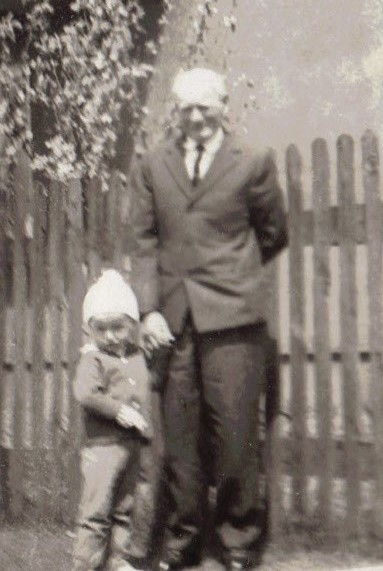
\includegraphics[width=0.4\textwidth]{zdjecia/jan_glab.jpg}
\caption[Jan Głąb z wnukiem Markiem Głąbem]{Jan Głąb, syn Walentego i Antoniny z domu Łyszczarz z wnukiem Markiem Głąbem, synem Jana}
\label{rys:jan_glab}
\end{center}
\end{figure}





\section{Antoni Głąb}
Antoni Głąb ożenił się dnia 23 IV 1960 r. w Sokolnikach z Ewą Śpiołek (ur. 8 lipca 1938 r. w Bliżycach z ojca Jana ur. 28 III 1903, zm. 1 V 1976 i matki Katarzyny z Wójcików ur. 27 IX 1908, zm. 5 I 1998), z którą ma dwójkę dzieci: Andrzeja Głąba (ur. 19 sierpnia 1961 r. w Myszkowie) oraz Elżbietę Głąbównę (ur. 22 grudnia 1962 r. w Myszkowie).


\begin{figure}[!h]
\begin{center}
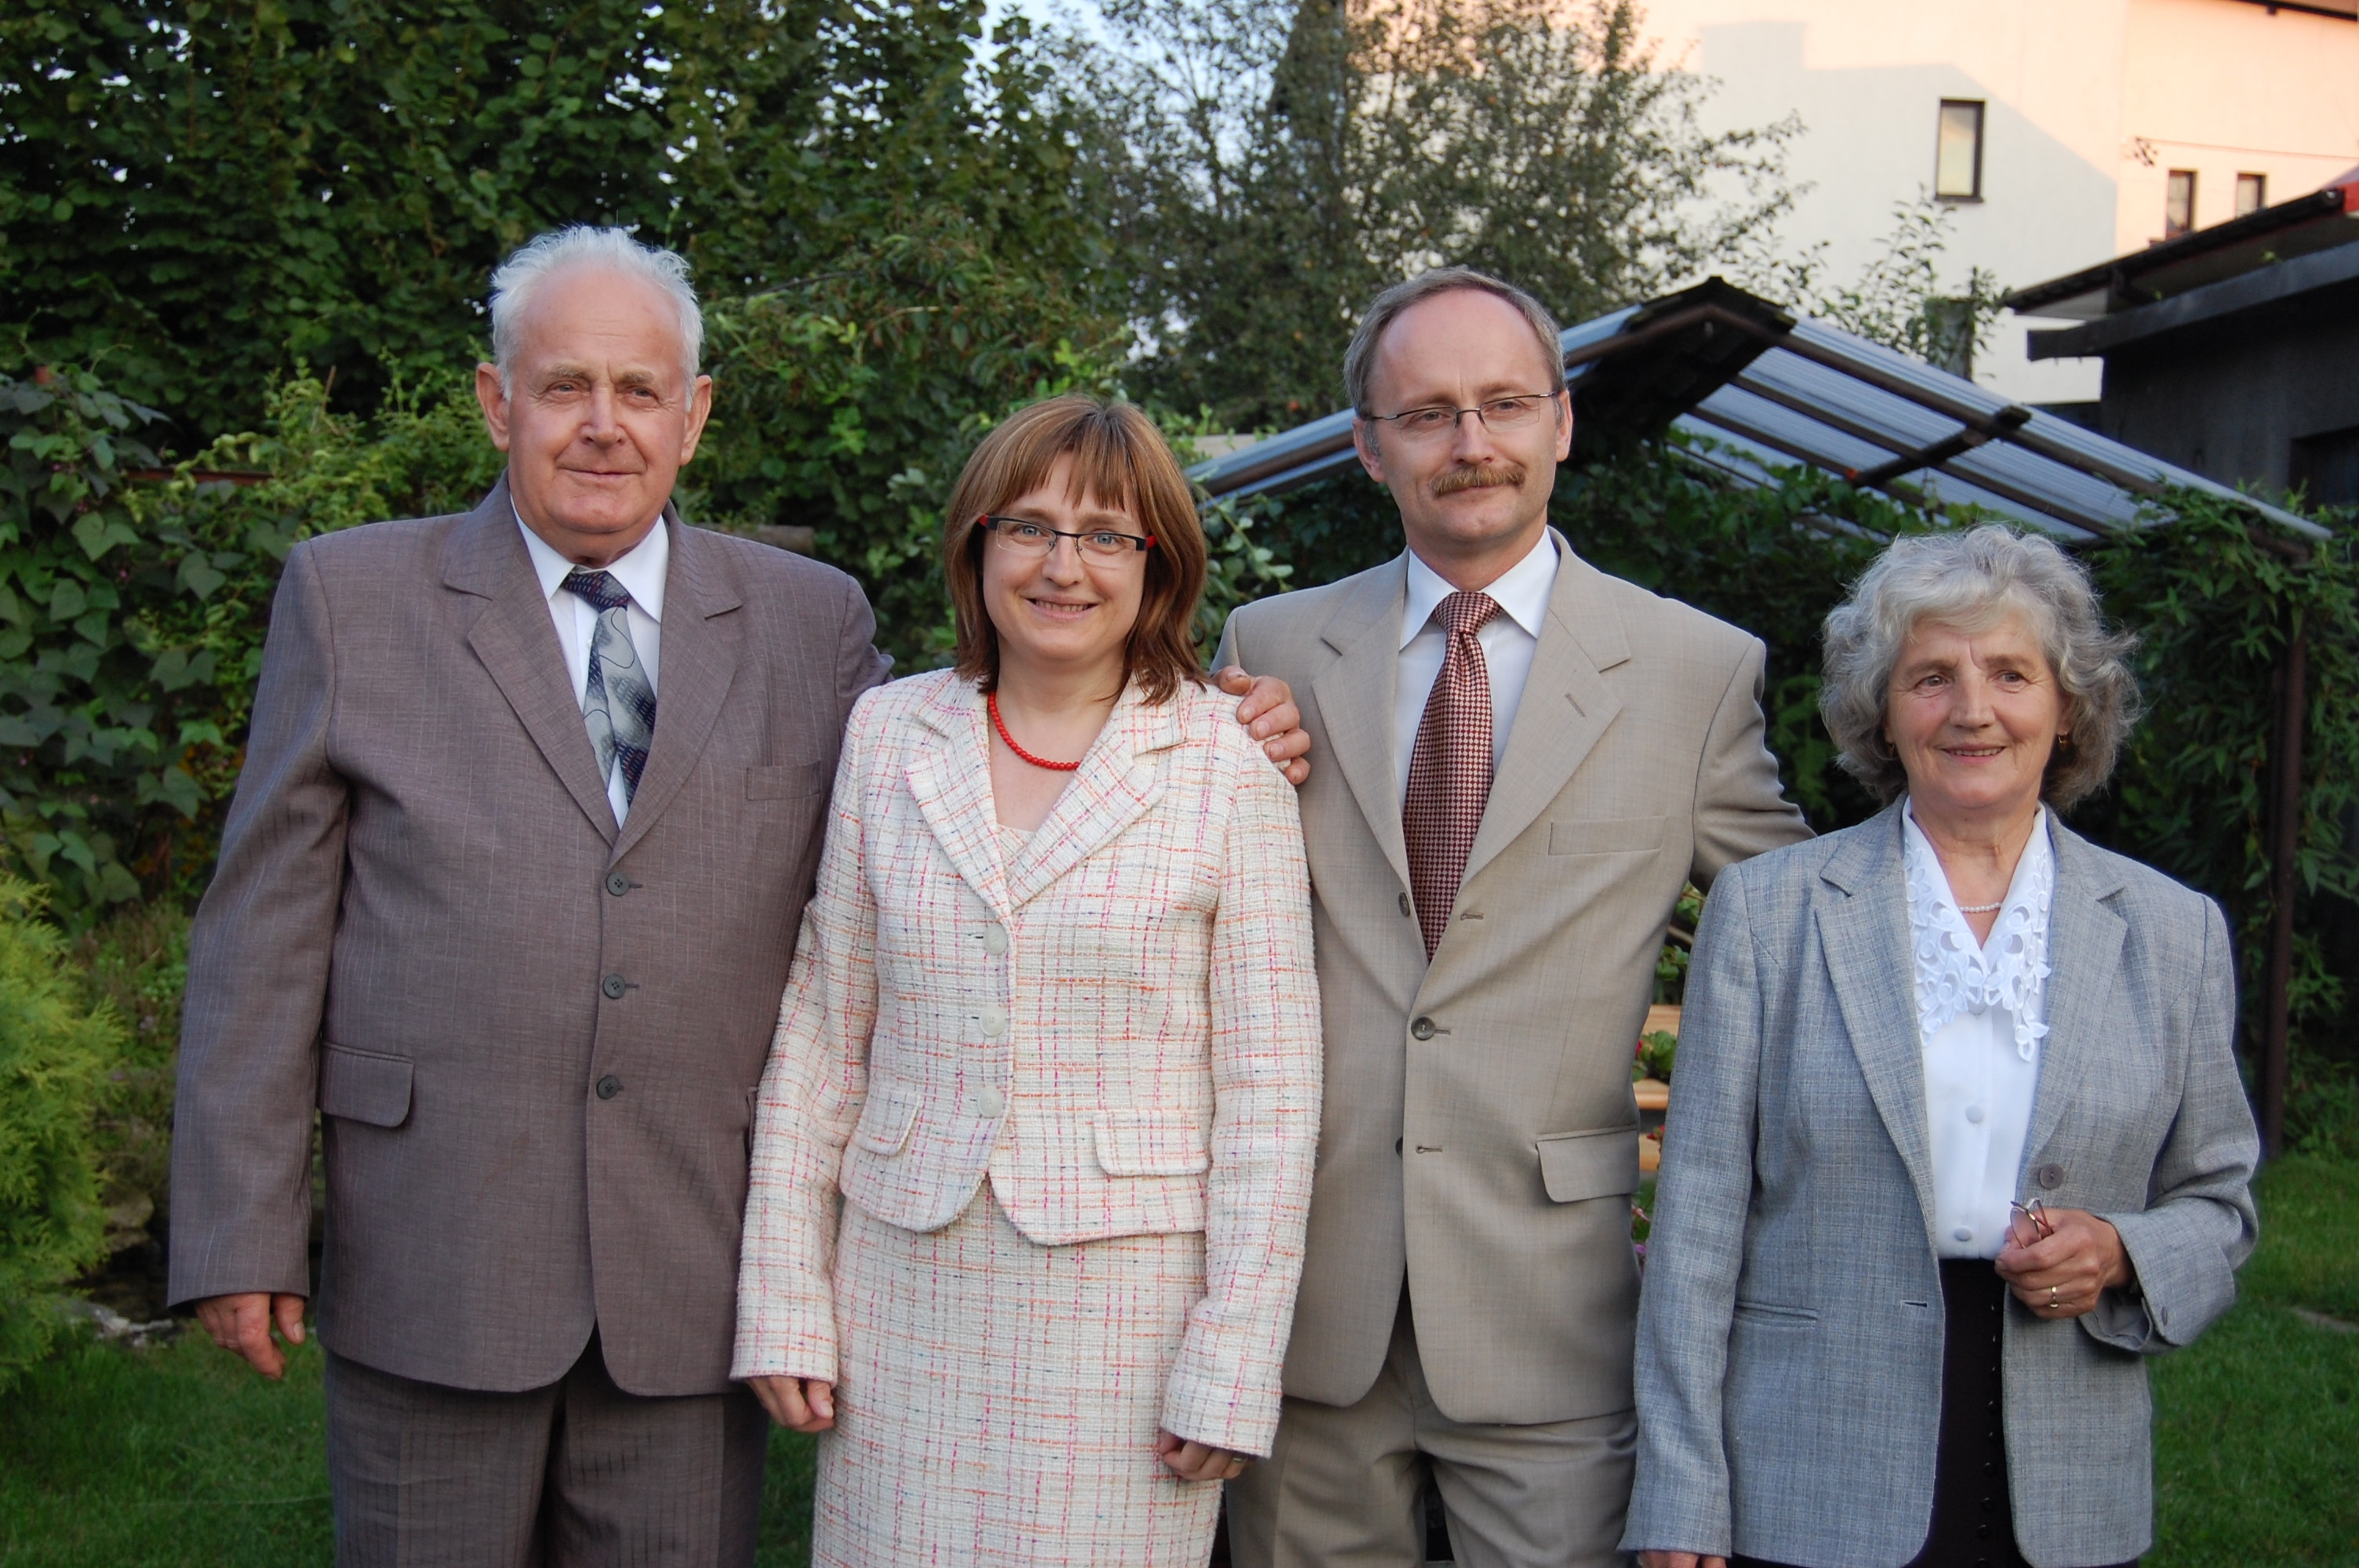
\includegraphics[width=0.6\textwidth]{zdjecia/ewa_antoni_glab_z_dziecmi.jpg}
\caption[Antoni Głąb z żoną i dziećmi]{Na zdjęciu od lewej: Antoni Głąb (najstarszy syn Jana), obok córka Elżbieta, dalej syn Andrzej i żona Ewa z domu Śpiołek}
\label{rys:ewa_antoni_glab_z_dziecmi}
\end{center}
\end{figure}

Andrzej ożenił się z Ewą Stankiewicz (ur. 10 grudnia 1960 r. w Łodzi z ojca Jerzego i matki Marii) i ma z nią syna Piotra (ur. 10 XI 1988 r. w Łodzi) oraz córkę Agatę (ur. XI 1990 r. w Łodzi). Gdy uzyskał dyplom lekarski zmienił nazwisko na Głąbiński. Obecnie jest profesorem zwyczajnym nauk medycznych na Uniwersytecie Medycznym w Łodzi w katedrze neurologii.

\begin{figure}[!h]
\begin{center}
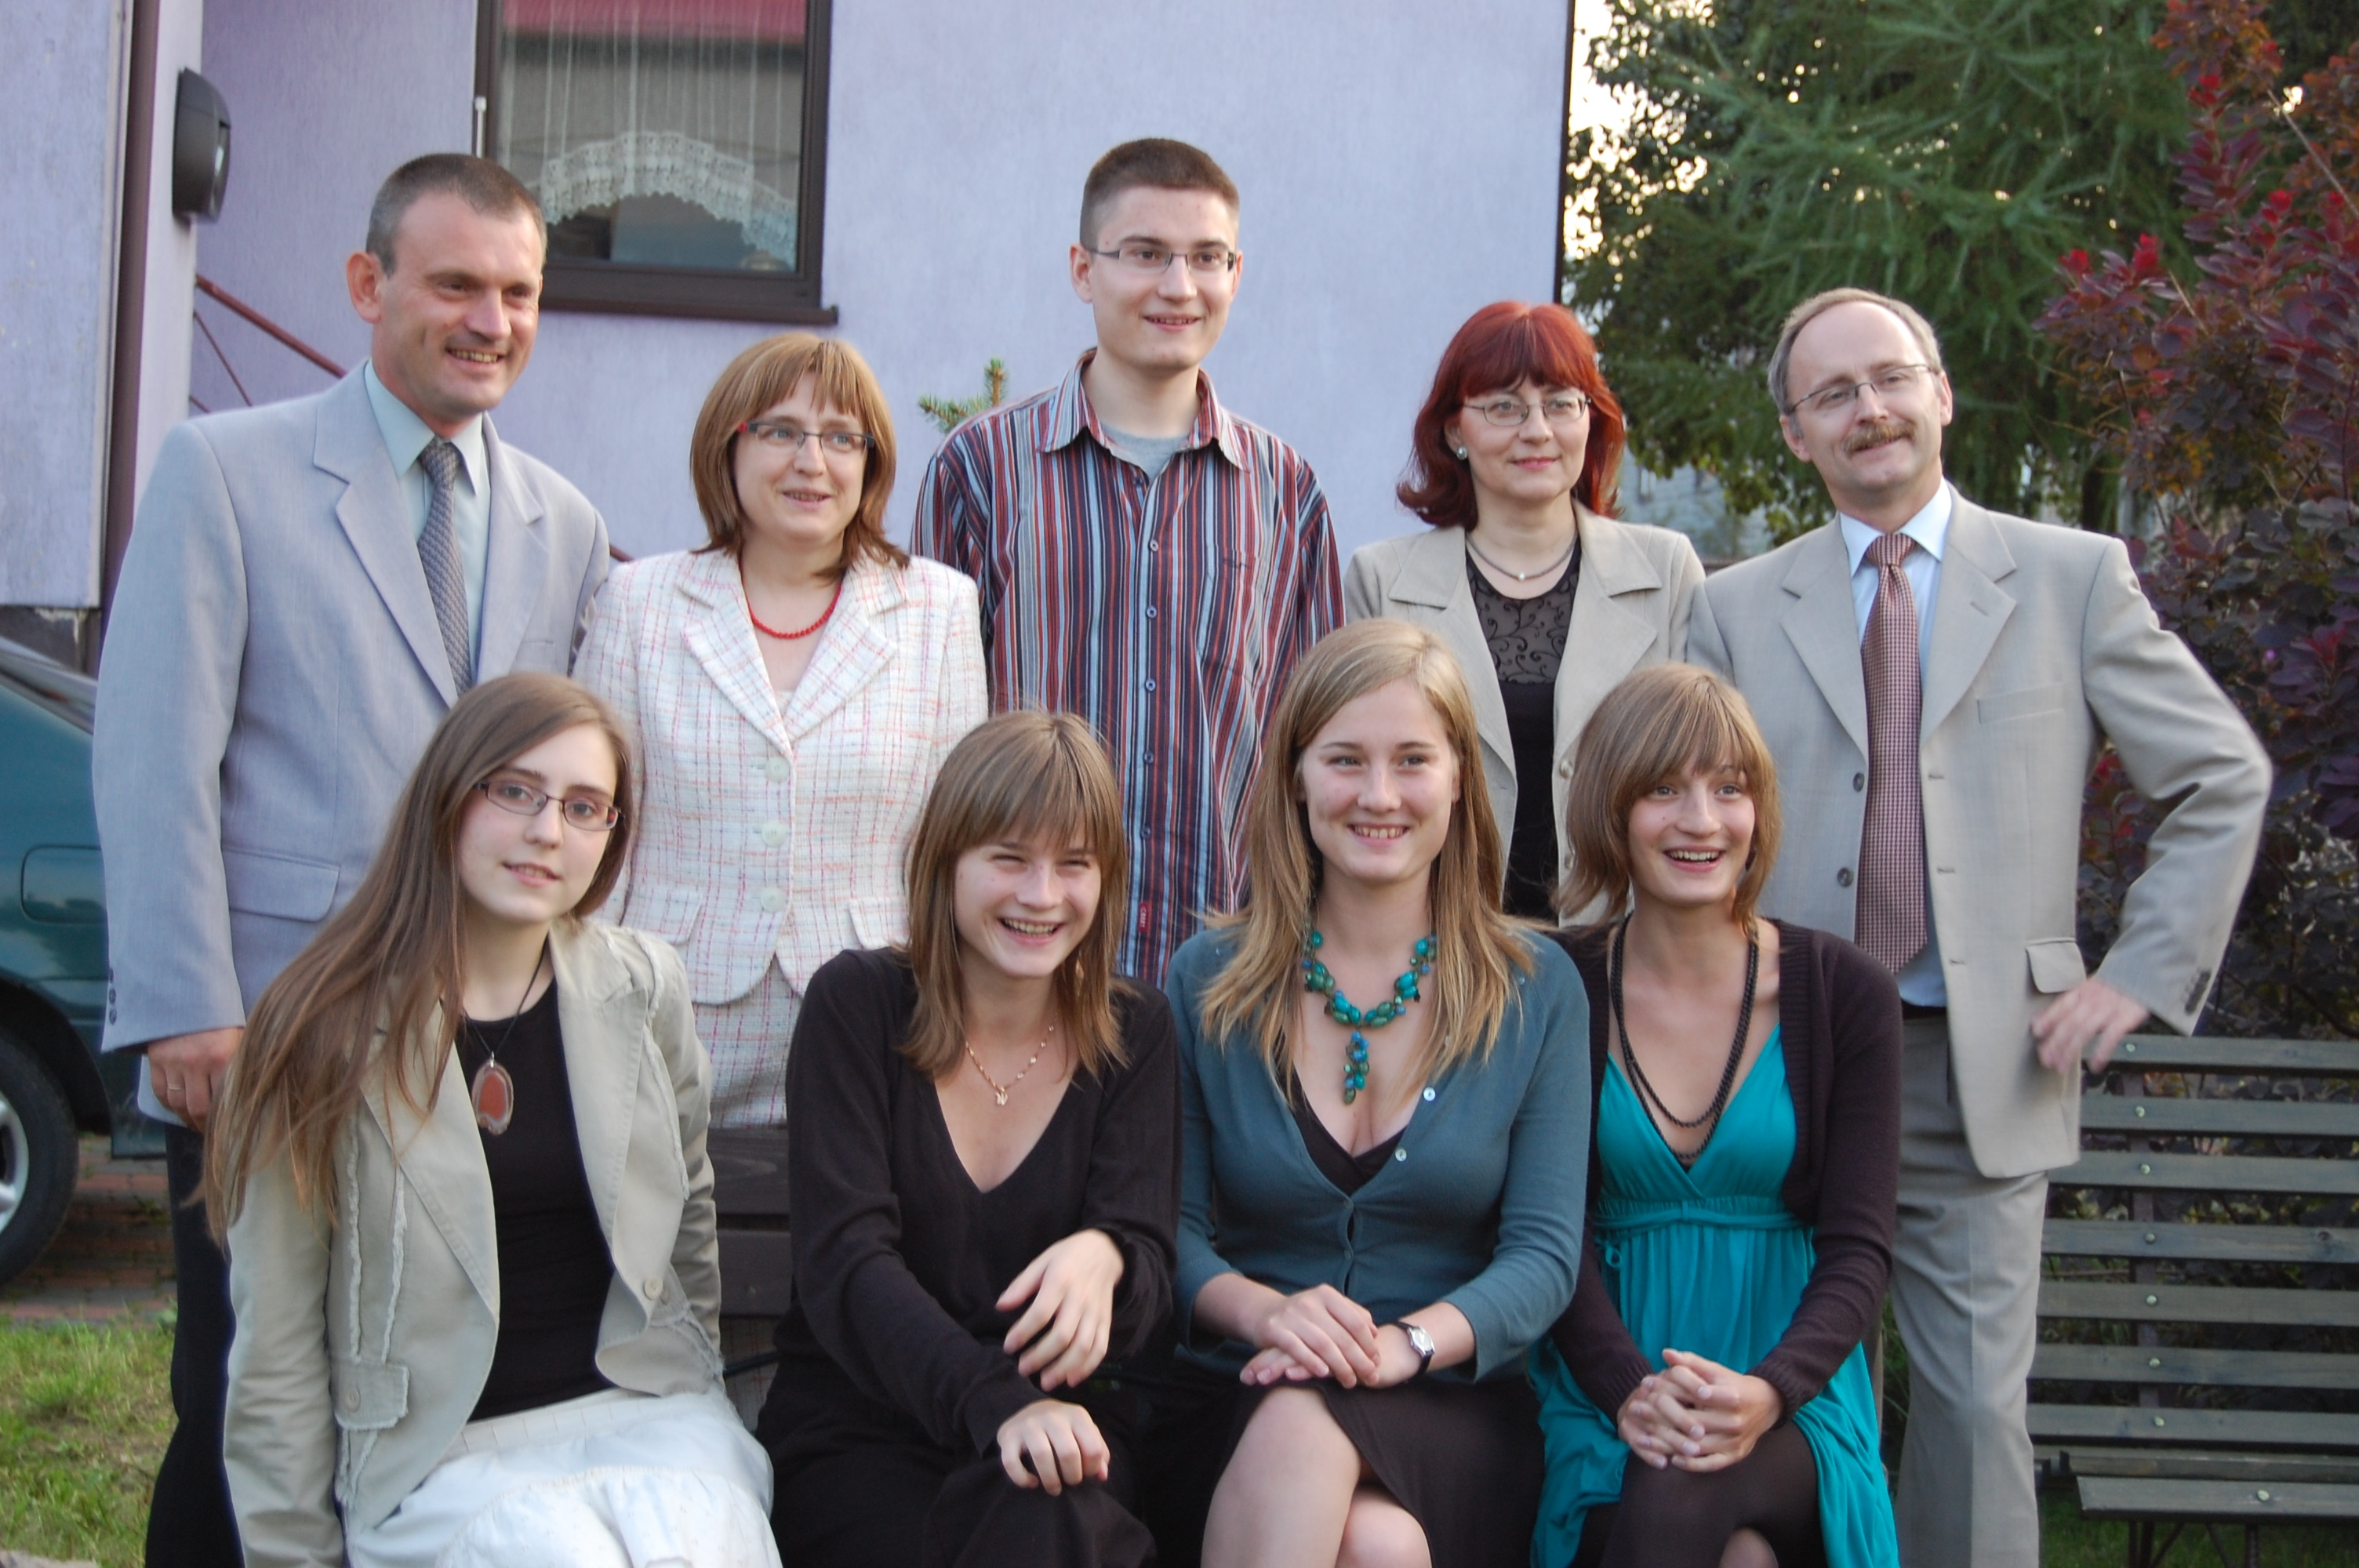
\includegraphics[width=0.7\textwidth]{zdjecia/elzbieta_anrzej_glab_z_dziecmi.jpg}
\caption[Elżbieta Doroszuk i Andrzej Głąbiński z rodzinami]{Na zdjęciu od lewej stoją: Andrzej i Elżbieta Doroszuk (z domu Głąb), w środku Piotr Głąbiński, syn Andrzeja, obok Ewa i Andrzej Głąbińscy. Poniżej siedzą: Agata Głąbińska, Weronika, Magda i Marta Doroszuk}
\label{rys:elzbieta_anrzej_glab_z_dziecmi}
\end{center}
\end{figure}

Jego siostra Elżbieta wyszła za Andrzeja Doroszuka (ur. 12 VI 1965 r. w Choszcznie z ojca Zbigniewa i matki Ireny ze Śmielewskich) i ma z nim trzy urodziwe córki: Magdalenę (ur. 23 XI 1988 r. w Krakowie) znakomitą tancerkę, Weronikę (ur. 19 VIII 1990 r. w Myszkowie) oraz najmłodszą Martę (ur. 11 I 1993 r. w Myszkowie).

Najstarsza z nich wyszła 11 VIII 2012 r. w Myszkowie w par. św. Ap. Piotra i Pawła za Daniela Deptułę (ur. 11 II 1987 r. w Szczytnie, syna Marka i Grażyny z Długołęckich).


\begin{figure}[!h]
\begin{center}
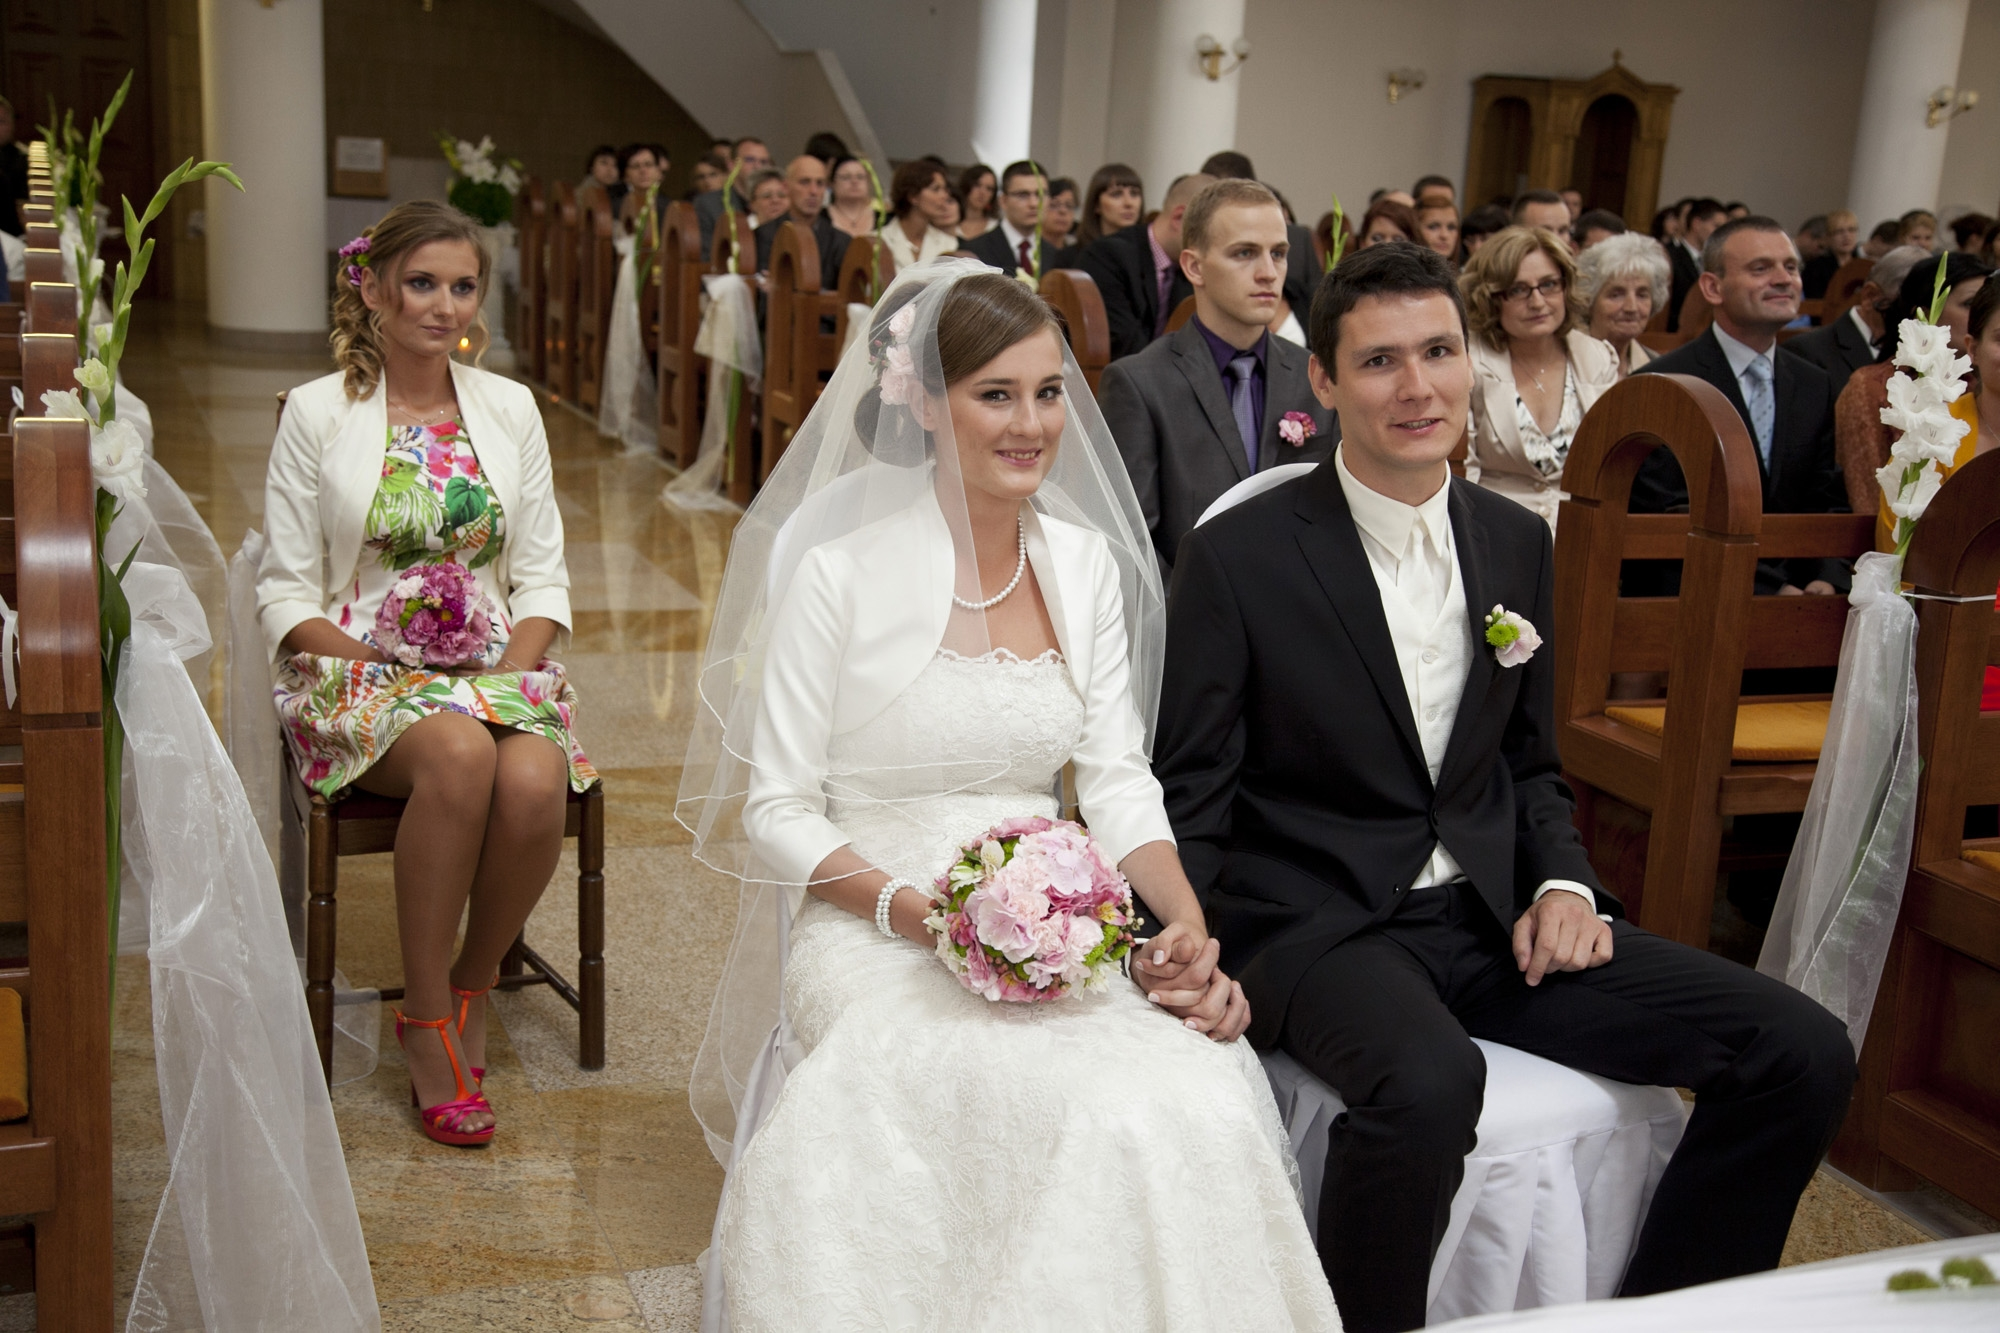
\includegraphics[width=0.6\textwidth]{zdjecia/slub_magdy_i_daniela_deptulow.jpg}
\caption{Ślub Magdy z domu Doroszuk z Danielem Deptułą}
\label{rys:slub_magdy_i_daniela_deptulow}
\end{center}
\end{figure}


\section{Maria Cecugiewicz z domu Głąb}

Maria Głąbówna (ur. 20 VI 1939 r. w Mirowie), córka Jana i Stanisławy wyszła dnia 11 IX 1960 r. w Niegowie za Eugeniusza Cecugiewicza (ur. 22 VI 1934 r. w Niegowie z ojca Zygmuta i matki Marii z domu Mędrek, zm. w 1979 r.).

\begin{figure}[!h]
\begin{center}
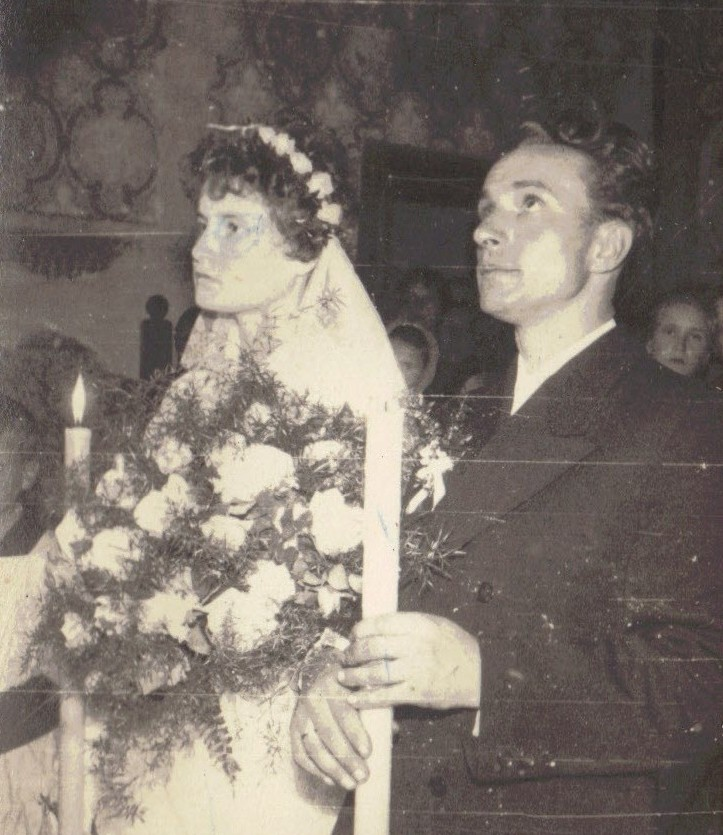
\includegraphics[width=0.45\textwidth]{zdjecia/slub_marii_i_eugeniusza_cecugiewiczow.jpg}
\caption{Ślub Marii z domu Głąb z Eugeniuszem Cecugiewiczem}
\label{rys:slub_marii_i_eugeniusza_cecugiewiczow}
\end{center}
\end{figure}

\begin{figure}[!h]
\begin{center}
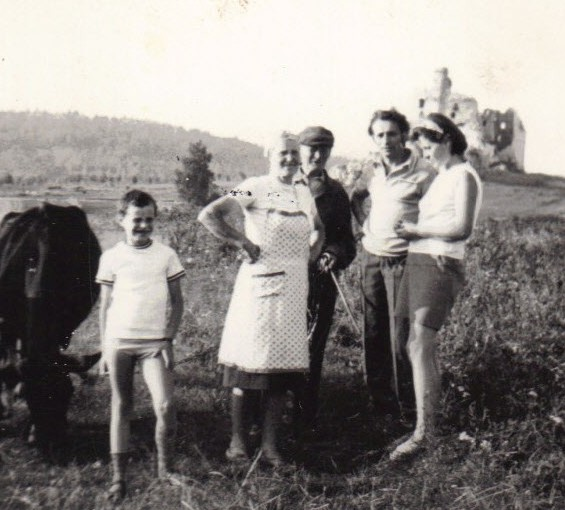
\includegraphics[width=0.55\textwidth]{zdjecia/maria_eugeniusz_cecugiewicz_z_rodzicami.jpg}
\caption[Maria i Eugeniusz Cecugiewicz z rodzicami]{Na zdjęciu od prawej: Maria (z domu Głąb) i Eugeniusz Cecugiewiczowie, dalej jej rodzice: Jan i Stanisława Głąbowie oraz bratanek Marek Głąb}
\label{rys:maria_eugeniusz_cecugiewicz_z_rodzicami}
\end{center}
\end{figure}

\begin{figure}[!h]
\begin{center}
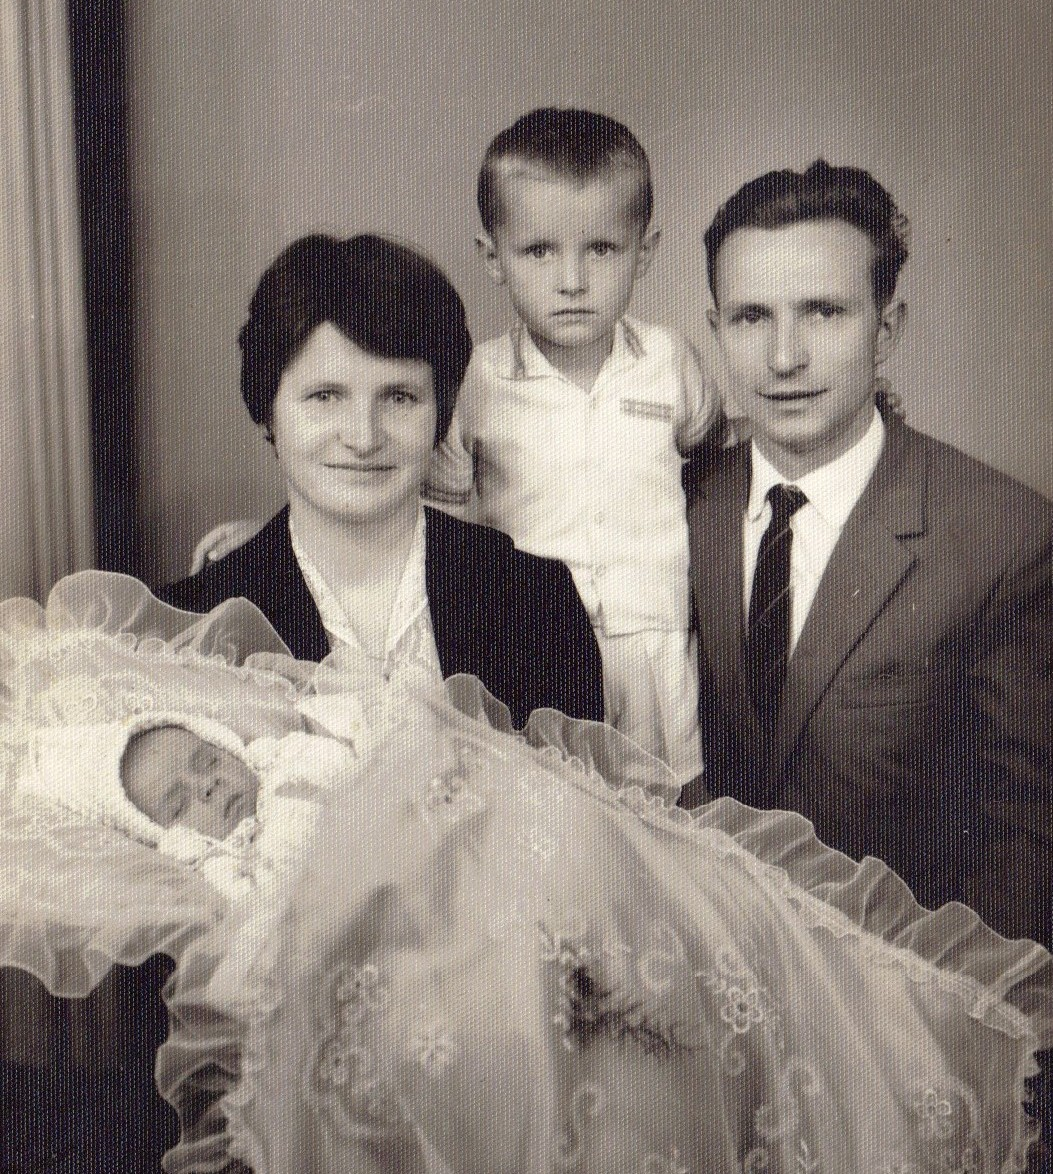
\includegraphics[width=0.45\textwidth]{zdjecia/chrzest_jerzego_cecugiewicza.jpg}
\caption[Chrzest św. Jerzego Cecugiewicza]{Chrzest św. Jerzego Cecugiewicza. Na zdjęciu rodzice: Maria i Eugeniusz Cecugiewiczowie, w środku brat Zdzisław}
\label{rys:chrzest_jerzego_cecugiewicza}
\end{center}
\end{figure}

Ma z nim dwóch synów Zdzisława (ur. 29 VI 1961 r. w Zawierciu) i Jerzego (ur. 28 V 1966 r. w Zawierciu).


\section{Jan Głąb}

Jan Głąb (ur. 1 I 1943 r. w Mirowie), najmłodszy syn Jana i Stanisławy, ożenił się dnia 2 X 1966 r. ze Zdzisławą Kurek (ur. 2 I 1947 r. w Mirowie z ojca Stanisława i matki Stanisławy Surowiec) i ma z nią syna Marka (ur. 27 VI 1967 r. w Zawierciu) oraz córkę Katarzynę (ur. 14 VII 1972 r. w Zawierciu).

\begin{figure}[!h]
\begin{center}
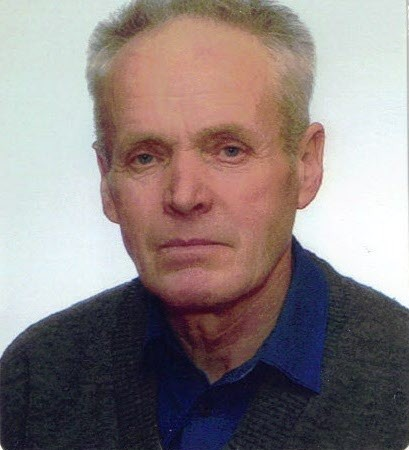
\includegraphics[width=0.35\textwidth]{zdjecia/jan_glab_junior.jpg}
\caption[Jan Głąb]{Jan Głąb, syn Jana, wnuk Walentego i Antoniny}
\label{rys:jan_glab_junior}
\end{center}
\end{figure}

\begin{figure}[!h]
\begin{center}
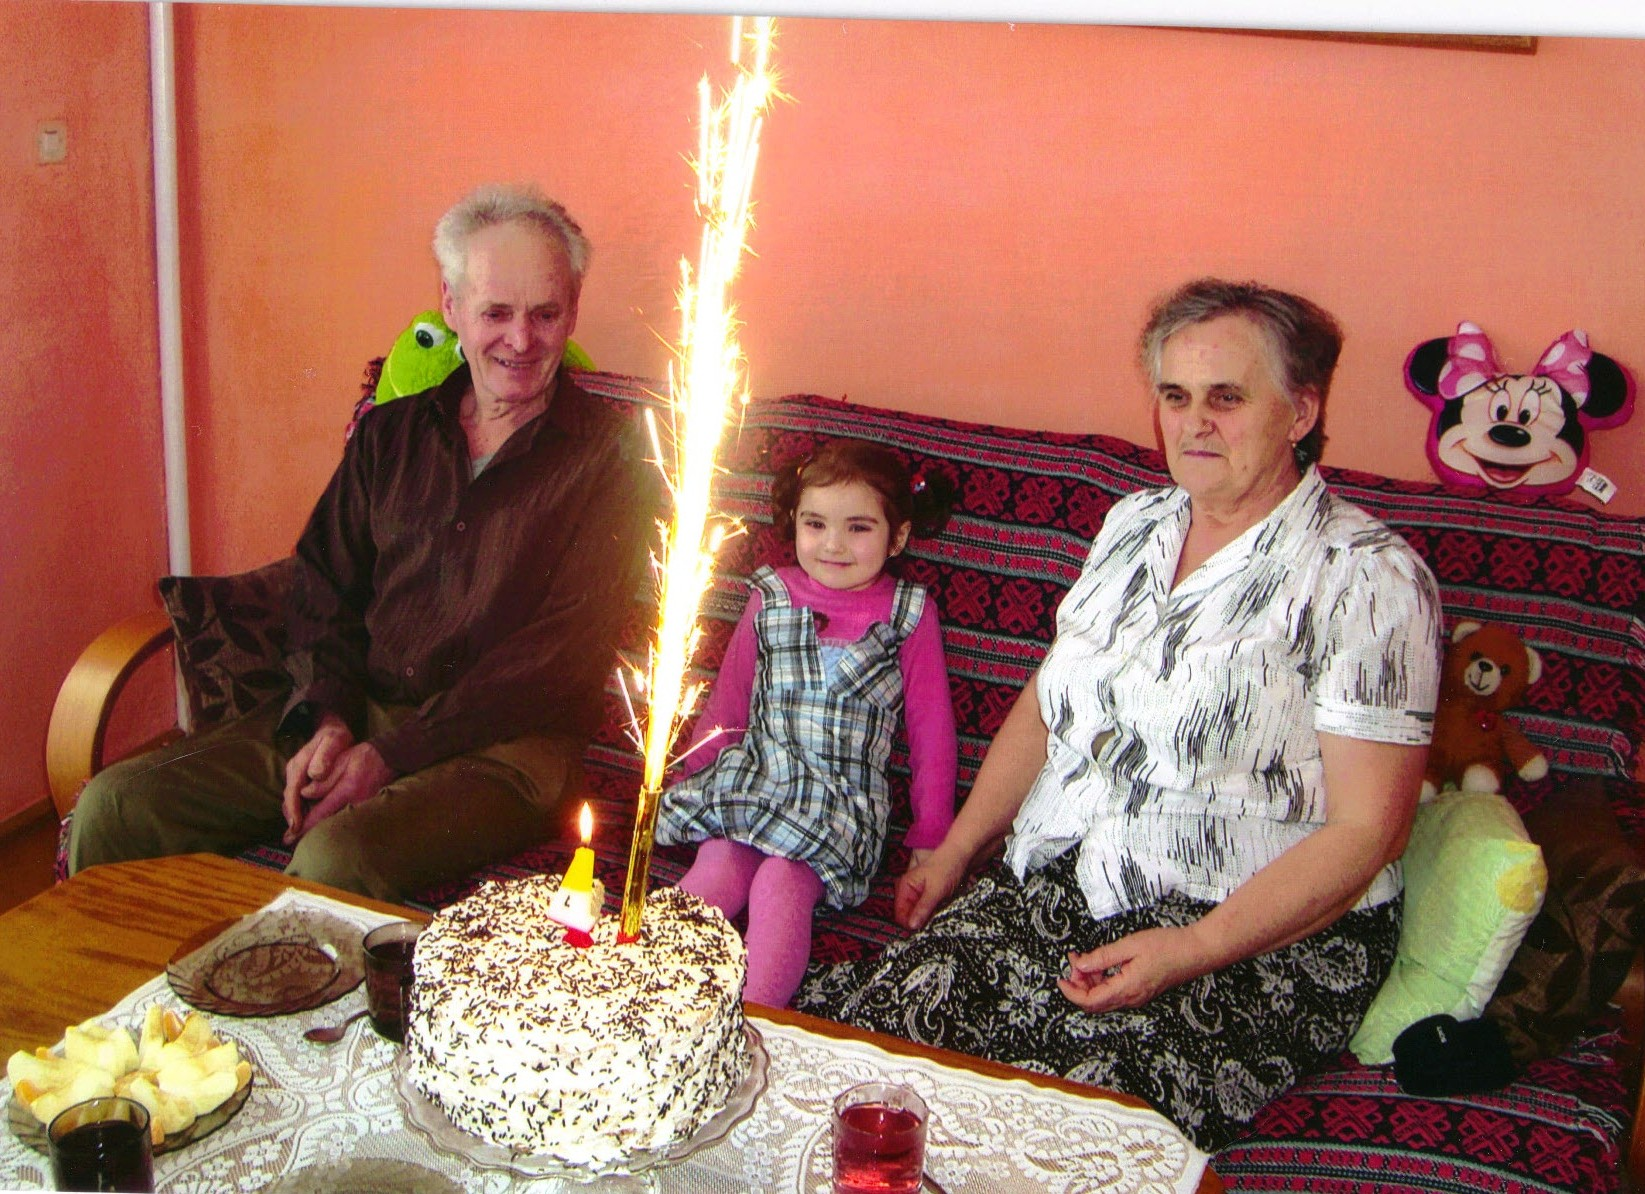
\includegraphics[width=0.6\textwidth]{zdjecia/jan_i_zdzislawa_glabowie.jpg}
\caption[Jan Głąb z żoną Zdzisławą z domu Kurek oraz wnuczką Zuzią]{Jan Głąb z żoną Zdzisławą z domu Kurek oraz wnuczką Zuzią (córką Katarzyny)}
\label{rys:jan_i_zdzislawa_glabowie}
\end{center}
\end{figure}

Marek Głąb ożenił się z Anną Muszyńską (ur. 31 V 1970 r. w Zawierciu) i ma z nią dwie córki: Karolinę (ur. 24 III 2000 r. w Zawierciu) i Amelię (ur. 31 V 2004 r. w Zawierciu).

\begin{figure}[!h]
\begin{center}
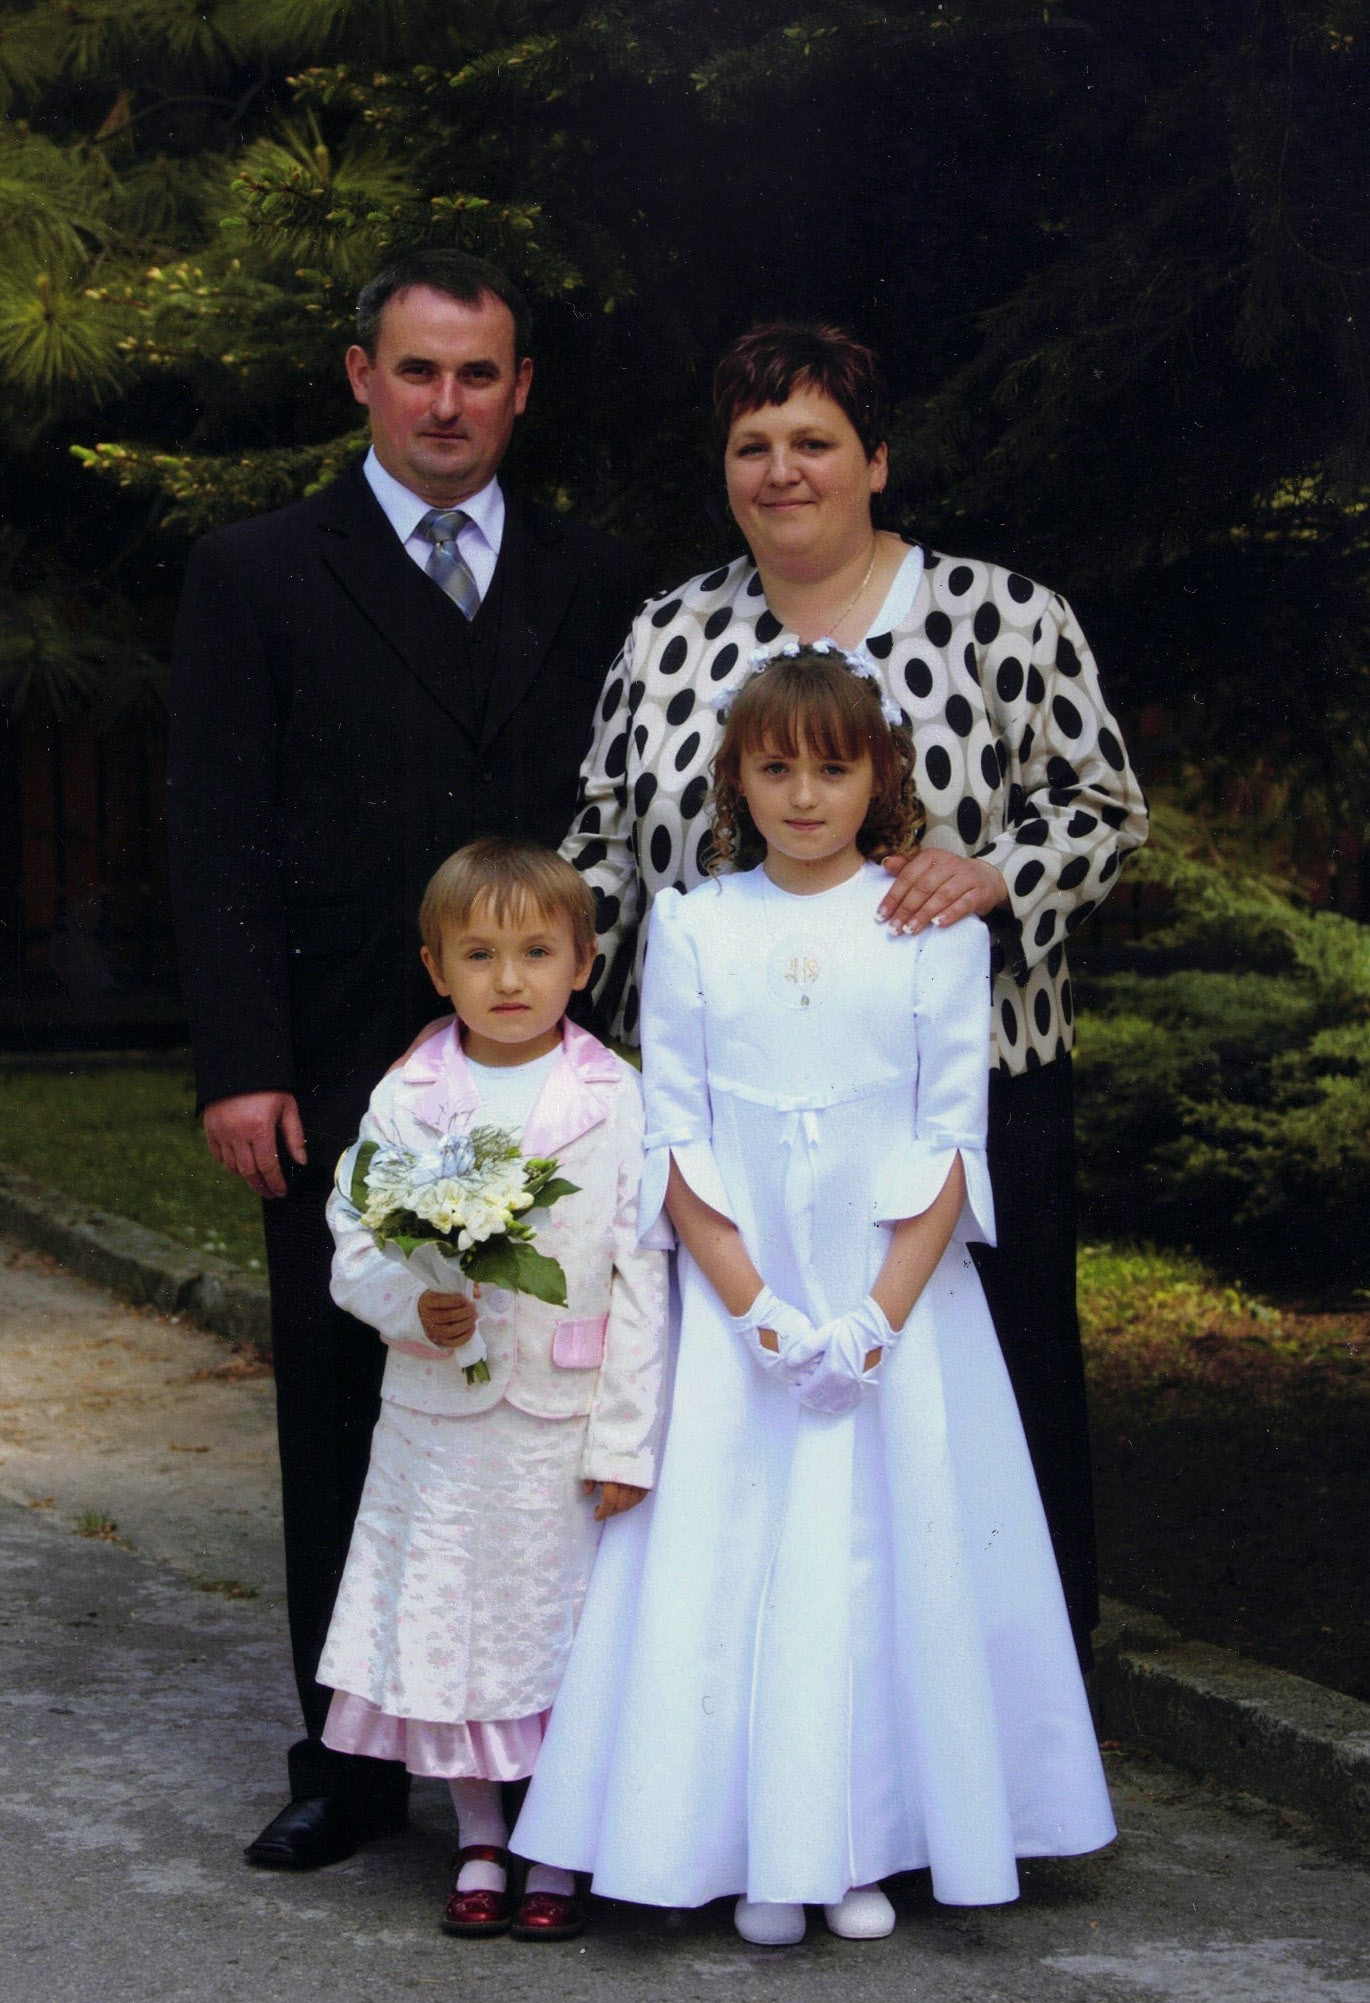
\includegraphics[width=0.4\textwidth]{zdjecia/marek_i_anna_glab_z_corkami.jpg}
\caption[Pierwsza Komunia św. Karoliny Głąb]{Pierwsza Komunia św. Karoliny Głąb. Na zdjęciu z rodzicami Markiem i Anną z domu Muszyńską oraz siostrą Amelią}
\label{rys:marek_i_anna_glab_z_corkami}
\end{center}
\end{figure}

Katarzyna Głąb, która ma swój wkład w gromadzeniu materiałów do niniejszej historii, cieszy się swą córką Zuzanną (ur. 23 II 2009 r. w Zawierciu).

\begin{figure}[!h]
\begin{center}
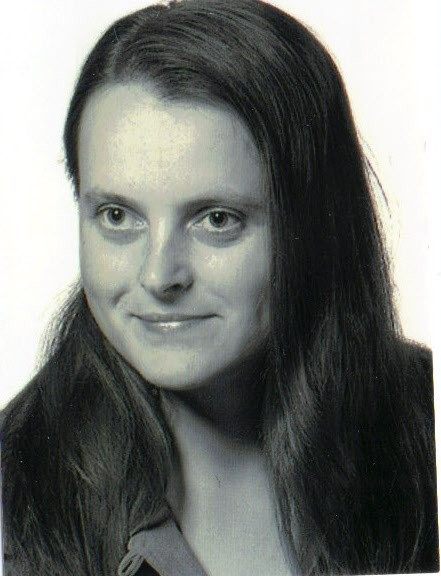
\includegraphics[width=0.35\textwidth]{zdjecia/katarzyna_glab.jpg}
\caption[Katarzyna Głąb]{Katarzyna Głąb - córka Jana i Zdzisławy}
\label{rys:katarzyna_glab}
\end{center}
\end{figure}

Nestorzy tej rodziny Jan i Stanisława Głąbowie żyli długo ciesząc się do końca dobrym zdrowiem (Jan zmarł 8 XI 1978 r. w Mirowie w wieku 80 lat, a jego żona Stanisława zmarła 21 marca 1998 r. w Mirowie w wieku 83 lat).

\begin{figure}[!h]
\begin{center}
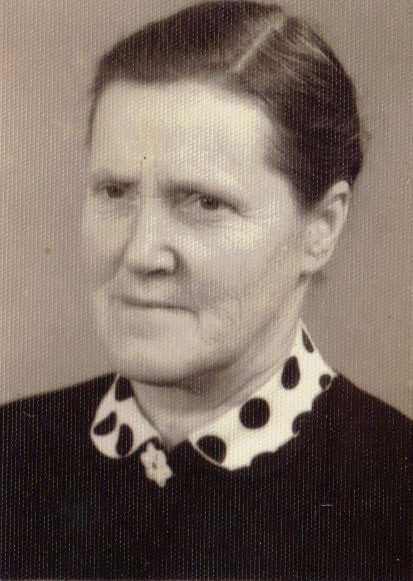
\includegraphics[width=0.35\textwidth]{zdjecia/stanislawa_glab.jpg}
\caption[Stanisława Głąb]{Stanisława Głąb z domu Machura - żona Jana}
\label{rys:stanislawa_glab}
\end{center}
\end{figure}

